\resizebox{!}{0.75\paperheight}{%
\begin{tikzpicture}

    % LOWER CHAMBER
    \foreach \i in {0,...,15}{
        \filldraw[color=black, fill=black!10, thick] (2*\i/3,     0*0.2) rectangle + (2*1/3, 0.2);
        \filldraw[color=black, fill=black!10, thick] (2*\i/3+1/3, 1*0.2) rectangle + (2*1/3, 0.2);
        \filldraw[color=black, fill=black!10, thick] (2*\i/3,     2*0.2) rectangle + (2*1/3, 0.2);
        \filldraw[color=black, fill=black!10, thick] (2*\i/3+1/3, 3*0.2) rectangle + (2*1/3, 0.2);
    }

    \filldraw[color=black, fill=black!10, thick] (0,      1*0.2) rectangle + (1/3, 0.2);
    \filldraw[color=black, fill=black!10, thick] (0,      3*0.2) rectangle + (1/3, 0.2);
    \filldraw[color=black, fill=black!10, thick] (2*16/3, 0*0.2) rectangle + (1/3, 0.2);
    \filldraw[color=black, fill=black!10, thick] (2*16/3, 2*0.2) rectangle + (1/3, 0.2);

    % LOWER SCINTILLATOR
    \filldraw[color=blue, fill=blue!10, thick] (17/3 - 2.5, 2.6) node[below left] {scintillator} rectangle + (5, 0.2);

    % ROTATED CHAMBER
    \foreach \i in {0,...,3}{
        \filldraw[color=black, fill=black!10, thick, opacity=0.7] (0, \i*0.2 + 2.9) rectangle + (2*1/3*16 + 1/3, 0.2);
    }

    % MIDDLE CHAMBER
    \foreach \i in {0,...,15}{
        \filldraw[color=black, fill=black!10, thick] (2*\i/3,     0*0.2 + 4.1) rectangle + (2*1/3, 0.2);
        \filldraw[color=black, fill=black!10, thick] (2*\i/3+1/3, 1*0.2 + 4.1) rectangle + (2*1/3, 0.2);
        \filldraw[color=black, fill=black!10, thick] (2*\i/3,     2*0.2 + 4.1) rectangle + (2*1/3, 0.2);
        \filldraw[color=black, fill=black!10, thick] (2*\i/3+1/3, 3*0.2 + 4.1) rectangle + (2*1/3, 0.2);
    }

    \filldraw[color=black, fill=black!10, thick] (0,      1*0.2 + 4.1) rectangle + (1/3, 0.2);
    \filldraw[color=black, fill=black!10, thick] (0,      3*0.2 + 4.1) rectangle + (1/3, 0.2);
    \filldraw[color=black, fill=black!10, thick] (2*16/3, 0*0.2 + 4.1) rectangle + (1/3, 0.2);
    \filldraw[color=black, fill=black!10, thick] (2*16/3, 2*0.2 + 4.1) rectangle + (1/3, 0.2);

    % UPPER SCINTILLATOR
    \filldraw[color=blue, fill=blue!10, thick] (17/3 - 2.5, 5) rectangle + (5, 0.2);

    % UPPER CHAMBER
    \foreach \i in {0,...,15}{
        \filldraw[color=black, fill=black!10, thick] (2*\i/3,     0*0.2 + 7) rectangle + (2*1/3, 0.2);
        \filldraw[color=black, fill=black!10, thick] (2*\i/3+1/3, 1*0.2 + 7) rectangle + (2*1/3, 0.2);
        \filldraw[color=black, fill=black!10, thick] (2*\i/3,     2*0.2 + 7) rectangle + (2*1/3, 0.2);
        \filldraw[color=black, fill=black!10, thick] (2*\i/3+1/3, 3*0.2 + 7) rectangle + (2*1/3, 0.2);
    }

    \filldraw[color=black, fill=black!10, thick] (0,      1*0.2 + 7) rectangle + (1/3, 0.2);
    \filldraw[color=black, fill=black!10, thick] (0,      3*0.2 + 7) rectangle + (1/3, 0.2);
    \filldraw[color=black, fill=black!10, thick] (2*16/3, 0*0.2 + 7) rectangle + (1/3, 0.2);
    \filldraw[color=black, fill=black!10, thick] (2*16/3, 2*0.2 + 7) rectangle + (1/3, 0.2);

    % ACTIVATED CELLS
    \filldraw[color=black, fill=red!40, thick] (2*7/3,      0*0.2) rectangle + (2/3, 0.2);
    \filldraw[color=black, fill=red!40, thick] (2*7/3+1/3,  1*0.2) rectangle + (2/3, 0.2);
    \filldraw[color=black, fill=red!40, thick] (2*7/3,      2*0.2) rectangle + (2/3, 0.2);
    \filldraw[color=black, fill=red!40, thick] (2*7/3+1/3,  3*0.2) rectangle + (2/3, 0.2);

    \filldraw[color=black, fill=red!40, thick] (2*8/3,      0*0.2 + 4.1) rectangle + (2/3, 0.2);
    \filldraw[color=black, fill=red!40, thick] (2*8/3+1/3,  1*0.2 + 4.1) rectangle + (2/3, 0.2);
    \filldraw[color=black, fill=red!40, thick] (2*8/3,      2*0.2 + 4.1) rectangle + (2/3, 0.2);
    \filldraw[color=black, fill=red!40, thick] (2*8/3+1/3,  3*0.2 + 4.1) rectangle + (2/3, 0.2);

    \filldraw[color=black, fill=red!40, thick] (2*9/3,      0*0.2 + 7) rectangle + (2/3, 0.2);
    \filldraw[color=black, fill=red!40, thick] (2*8/3+1/3,  1*0.2 + 7) rectangle + (2/3, 0.2);
    \filldraw[color=black, fill=red!40, thick] (2*9/3,      2*0.2 + 7) rectangle + (2/3, 0.2);
    \filldraw[color=black, fill=red!40, thick] (2*8/3+1/3,  3*0.2 + 7) rectangle + (2/3, 0.2);

    % MUON TRACK
    \draw[color=red, very thick] (17/3-0.6, -0.5) -- (17/3+0.7, 8.3) node[right] {muon track};


    \node(cell) at (17/3-2, -3) {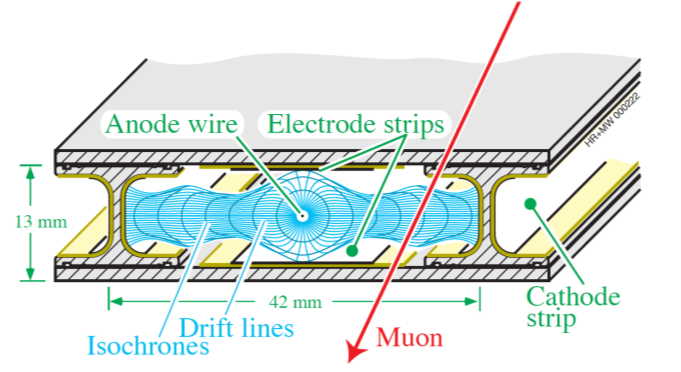
\includegraphics[width=1.4\textwidth]{./Images/cell.png}}; 
    
    \draw[bend left,<-, very thick, shorten <=2pt, shorten >=2pt] (cell) to node[midway,right] {drift tube} (1/3,0.1) ;

    \node(eq)[below right = -3cm and 0.5cm of cell, scale=2, rectangle, fill=yellow!50] {$x=\pm \,
    v_{\text{drift}}\,\underbrace{(t-t_0)}_{\text{\alert{drift time}}}$};
         
\end{tikzpicture}
}